\section{Introduction}

Many programmers develop code by interleaving opportunistic information foraging with writing code~\cite{brandt_two_2009}\cite{brandt_example-centric_2010}.
When learning about unfamiliar technologies, programmers start by searching for tutorial web sites.
Instead of examining the prose, they experiment with code examples, using source code from the pages to support learning by doing~\cite{brandt_two_2009}.
However, programmers of all backgrounds~\cite{duala-ekoko_asking_2012,dorn_lost_2013,dorn_learning_2010} struggle to leverage web documentation to solve programming problems.

One source of confusion is that authors write learning materials with a certain audience in mind.
This intended target audience determines what information is included, and what is omitted.
For example, an author of a tutorial on web scraping may expect users to be familiar with Python, CSS selectors, regular expressions, and threads.
However, members of the actual audience may have different skills.
It is impractical for the author to introduce all relevant parts of each language in detail.
As a result, today's Q\&A sites like StackOverflow and tutorial-style blogs lack immediate scaffolding for readers seeking clarification on unfamiliar or complex syntax. 

\begin{figure}[!t]
\centering{
    \subfigure[A \gls{exp} with automatically generated natural language explanation of a CSS selector and a demonstration of an HTML element it matches.]{
        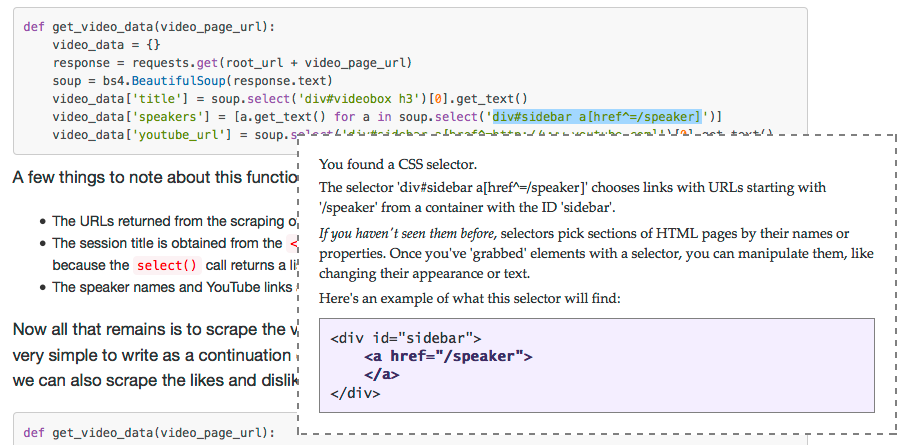
\includegraphics[width=\columnwidth]{figures/accelerator_css}
        \label{fig:accelerator_css}
    }
    \subfigure[A \gls{exp} describing the high-level intent and low-level argument values of a \texttt{wget} command line.]{
        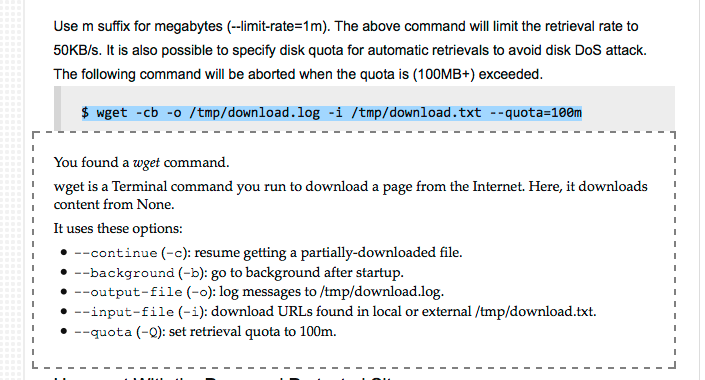
\includegraphics[width=\columnwidth]{figures/accelerator_wget}
        \label{fig:accelerator_wget}
    }
    \caption{
    \Gls{name}-generated \glspl{exp} enable programmers to seek in-situ help when reading and adapting code found in online tutorials and Q\&As.
    Programmers select the code they want clarification about, and view natural language descriptions and demonstrations of what the code does.
    }
    \label{fig:accelerators}
}
\end{figure}

\begin{changes}
One of the attributes of recognized answers on StackOverflow, according to Nasehi et al.~\cite{nasehi_what_2012}, is step-by-step solutions.
A step-by-step solution is presented in a detailed and ordered fashion, in a simple way, in a way that's familiar to the questioner or friendly to newcomers.
Answers with this attribute sometimes provide a simulation of what the code does, or describe multiple elements needed to perform a single programming task. \if 0
Three common attributes of low-vote answers on StackOverflow (lack of explanation, in addition to lack of code and shortcomings of solution).
This implies that some code examples could be more valuable to programmers looking for online inspiration if their explanations were complete and at the appropriate level of detail~\cite{nasehi_what_2012}.
\fi
The routines we develop here enable step-by-step explanations and simulations of existing code to add value to existing code examples.
\end{changes}

To provide the missing scaffolding for unexplained code in tutorials, Q\&As, and other online programming help, we propose routines called \emph{\Glspl{name}} that produce on-demand, context-relevant descriptions of code from domain-specific languages and commands.
\Glspl{name} automatically find pieces of code in webpages and augment these with \glspl{exp}.
These explanations are \emph{on-demand} --- they can describe code found anywhere, to provide just-in-time understanding of code.
They are also \emph{context-relevant}, describing only the syntactic elements that are present and important within a snippet, in domain-specific terms.
This distinguishes these explanations from getting-started guides and reference documentation for a language by minimizing the amount of text programmers have to reference to understand source code.

\if 0
We draw on inspiration of layered documentation to justify our current work. \appachu{one liner to describe layered documentation}
Decades of research on technical communication provide best practices for writing usable documentation.
In the domain of software, minimalist instruction~\cite{carroll_nurnberg_1990} recommends enabling users to start immediately on realistic tasks, minimizing the necessary  reading and other passive activity, and supporting error recognition and recovery.
Farkas ~\cite{farkas_layering_1998} introduces layered documentation as an extension to minimalist instruction that enables users from different backgrounds to benefit from the same documents by providing optional backup information for tasks like error recognition and correction.
\fi 

Such explanations can describe languages like CSS selectors, regular expressions, and terminal commands (see Figure~\ref{fig:accelerators}).
\Glspl{name} are programmed to detect relevant code, parse it, and generate natural language explanations and demonstrations of code. 
In our own implementation, each language can be supported in several hundred lines of code.
We show that they can be built as standalone servers, accessible by an addon in the programmer's browser to provide just-in-time explanations of a language or command anywhere on the web.
With the \glspl{name} that we build for CSS selectors, regular expressions and command lines, we show an expanse of domain-specific representations of code, from natural language to example HTML DOMs.

Our contributions are as follows.
First, we introduce a framework for building \Glspl{name}, generators of natural language explainations and demonstrations for domain-specific languages and command lines.
Second, we demonstrate the processing pipeline, technical considerations, and design guidelines involved in build \glspl{name} through our efforts to implement them for CSS selectors, regular expressions, and command lines.
Finally, we show through an in-lab study how \gls{name}-generated explanations can help programmers modify existing code containing CSS selectors and wget commands without referring to external documentation.